\chapter{Getting Started with OMPL.app}
\label {chp:ompl.app}

OMPL.app provides a graphical front-end to the core OMPL library, and allows
a user to see many of the ideas from sampling-based motion planning in action.
The GUI is written using Python and PyQt.  OMPL.app comes bundled with
the core OMPL library, and can be found at {\tt ompl.kavrakilab.org}.

By using OMPL.app, introductory users to OMPL can get a sense of the current
capabilities of the library and sampling-based motion planning.  As of version
0.9.5, users can use geometric motion planning for rigid bodies in 2D and 3D,
control a variety of simplified kinodynamic systems (e.g. unicycle, blimp, or car),
and even a dynamic car using the Open Dynamics Engine.  OMPL.app
also demonstrates one possible way of representing the geometry of the robot
and how to provide collision checking to the core library using a particular
geometric representation.

\section {Using OMPL.app}

To launch OMPL.app, execute the {\tt ompl\_app.py} python script, which is found
in the {\tt omplapp/ gui} directory.  When the GUI is loaded, a window will be
presented as in figure \ref{fig:omplapp:start}.

\begin {figure}[h]
\centering
{
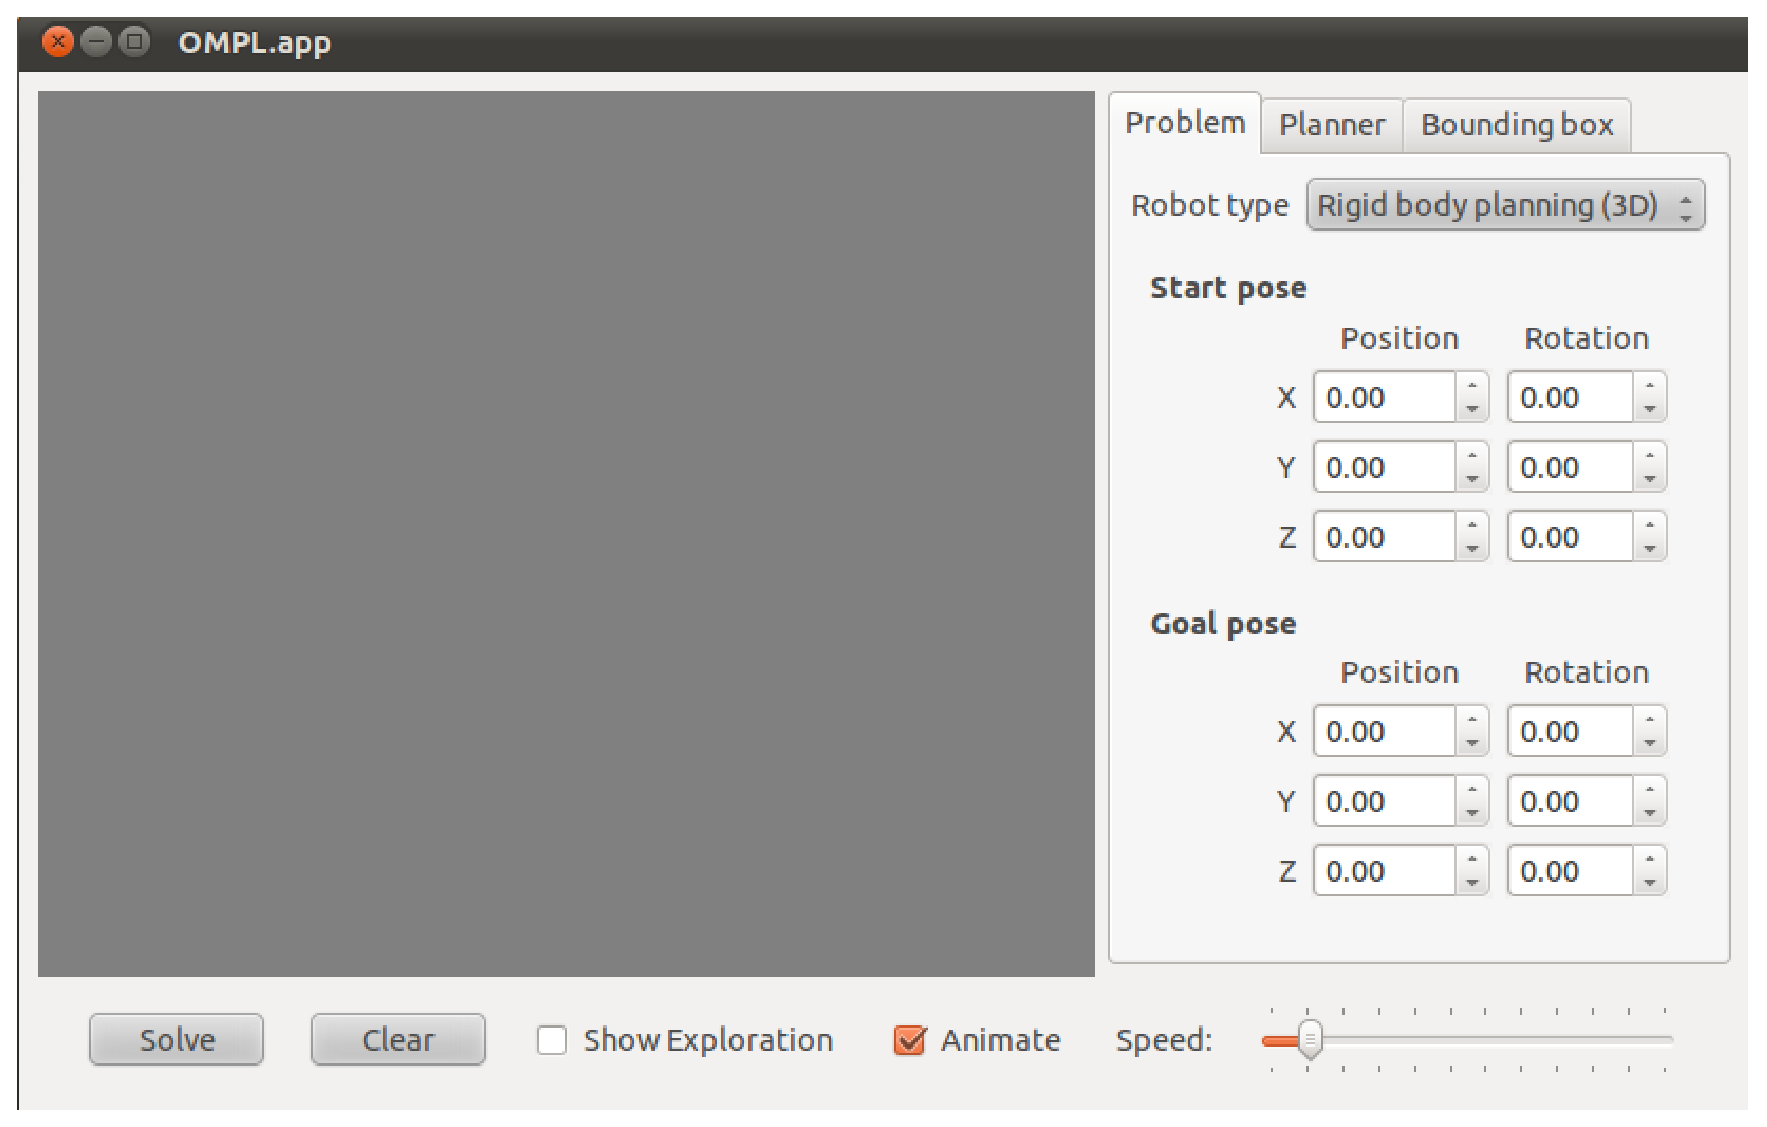
\includegraphics [width=3.5in]{omplapp_start}
\caption {OMPL.app at startup}
\label {fig:omplapp:start}
}
\end {figure}


OMPL.app requires us to do 3 things to solve a motion planning query: setup the
workspace and the robot, select a planner to use, and bound the environment.
These three items correspond to the tabs located in the upper right portion of
the window.

\subsection {Selecting a Robot and Environment}
First, a robot type must be selected.  The traditional ``piano mover's'' problem
is a rigid body planning in 3D instance, so select ``Rigid body planning (3D)''.
Next, the environment and the robot itself must be loaded.  OMPL.app comes
packaged with a number of mesh models for 2D and 3D environments and robots.
Go to the {\it File} menu at the top of the window and select
{\it Open Environment}.  This presents a dialog screen to open a file.  Navigate
to the {\tt omplapp/resources/3D} directory and select the {\tt Easy\_env.dae}
mesh to load.  Then select {\it Open Robot} from the file menu and open
{\tt Easy\_robot.dae} from the same directory.  When the meshes are loaded, you
will see an environment consisting of a wall partitioning the space into two
parts with a small opening in the center (figure \ref{fig:omplapp:easy}).
Rotate the view using the mouse to see both sides of the partitioned space and
the ``L'' shaped robot inside the opening of the wall.

\begin {figure}[h]
\centering
{
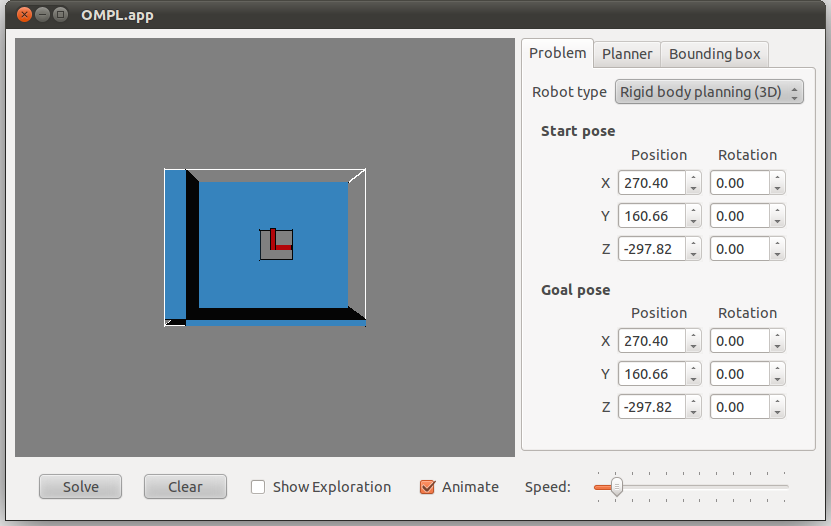
\includegraphics [width=3.5in]{omplapp_easy}
\caption {The ``easy'' environment loaded with the robot occupying the opening.}
\label {fig:omplapp:easy}
}
\end {figure}

Next the start and goal configurations must be chosen.  When a robot mesh is
first loaded, the start and goal poses are equivalent.  In the ``easy''
environment, the most interesting queries involve the robot maneuvering through
the opening in the wall.  One such configuration is $(270, 50, -200)$ and $(270,
50, -400)$, respectively.  Set the start and goal positions to these values and
click ``Solve'' to find a solution with the default planner.  The
default planner shouldn't have too much trouble solving this query.  When a
solution is found the robot will become animated and travel along the computed
path.  If the planner fails to find a solution, repeat the solving process
until one is found.

The user can also switch between an animated robot and a view of the discrete
segments of the path by toggling the ``Animate'' check box.  Also, a
projection of the random samples can be seen by checking the ``Show
Exploration'' box.  In a bi-directional planner, the samples from each direction
will be shown as different colors.

\begin {figure}[h]
\centering
{
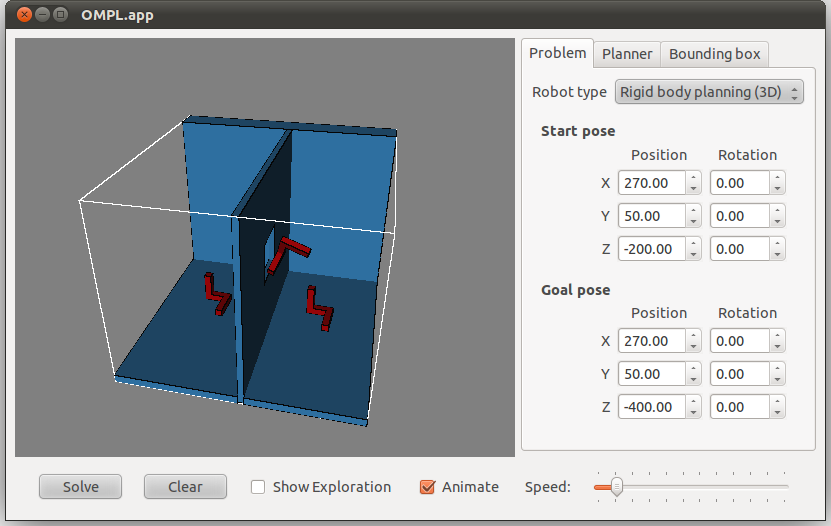
\includegraphics [width=3.5in]{omplapp_easy_sln}
\caption {The ``L'' shaped robot moving through the narrow passage.}
\label {fig:omplapp:easysolution}
}
\end {figure}

\subsection {Choosing a Planner}
Due to the wide variety in how sampling-based planners operate, selecting a
different planner may yield better results for a specific query.  Moreover,
the amount of time allotted to the planner can be customized.  In geometric
instances, the collision checking resolution that is employed by the local
planner can be changed to improve performance.  For instances that use motion
controls, the propagation step size for each control can be specified, as
well as the range of possible steps to apply the control.  In addition to these
general parameters, many of these methods have parameters that can be tuned
to further improve the time needed to solve a query and/or the quality of the
solution returned.  OMPL.app exposes these parameters, many of which are common
amongst the various planners, under the ``Planner'' tab.  The following defines
the most common parameters seen in geometric and control based planners in OMPL:

\begin{description}
\item[Range:] This parameter represents the maximum length of a motion
to be added in the tree of motions. It greatly influences the runtime of the
algorithm.

\item[Goal bias:] In the process of randomly selecting states in the state
space to attempt to go towards, the algorithm may in fact choose the actual goal
state with some probability. This probability is a real number between 0.0 and
1.0; it should not be too large, and usually lies around 0.05.

\item[Border fraction:] Planners such as {\tt KPIECE} use a discretization
of a projection of the state space to guide the exploration. This discretization
consists of a set of cells. The border fraction is the fraction of time spent
focusing the exploration on border cells (cells at the exploration ``frontier'').
This represents the minimum percentage used to select cells that are on the
border (minimum because if 95\% of cells are on the border, they will be
selected with 95\% chance, even if the border fraction is set to 0.9 (90\%)).

\item[Max.\ nearest neighbors:] The maximum number of nearest neighbors for
which a connection will be attempted when a new configuration sample is added.
\end{description}

Every effort is made to set the defaults for these settings to values that are
conducive in general planning environments.  However, depending on the
difficulty of the query, these settings may need to change to yield better
performance.  Consult the literature for the different planners to understand
how changing a specific parameter will change the behavior of a method in a
particular instance.

\subsection {Bounding the Environment}
By default, the robot is constrained to move inside a tight bounding box around
the environment, the start pose, and the goal pose. The bounding box is
visualized in OMPL.app as the white frame around the environment and robot.
These bounds apply to a reference point for the robot; the origin of the
coordinate frame that defines its pose. This means that parts of the robot can
stick outside the bounding box. It also means that if the reference point for
your robot is far away from the robot itself, you can get rather unintuitive
results. The reference point is whatever the origin is in the mesh; OMPL.app is
not using the geometric center of the mesh as the reference point.

\subsection {Saving and Replaying Solution Paths}
OMPL.app also has the ability to save the current solution path and reload that
path for viewing in the future.  Once a problem has been solved, the solution
found can be saved to a text file by selecting ``Save Path'' from the File menu.
A save dialog will be presented to select a directory and filename to save the
path to. Similarly, the path can be reloaded and replayed by selecting ``Load
path'' from the File menu.  The environment or robot mesh data is not saved in
this path file.  The same environment and robot must be reselected by the user
to replay the same path.

\section {OMPL.app vs.\ OMPL}
OMPL.app builds upon the motion planning functionality in OMPL by specifying
a geometric representation for the robot and its environment, and provides
a collision checking mechanism for the representation to the existing planners
in the library.  Specifically, OMPL.app utilizes PQP \cite{Larsen:2000} by
default for collision checks, but also provides a wrapper for FCL
\cite{Jia:2011} collision checking as well. The core Open Motion Planning
Library does not explicitly represent the robot or the environment, and it is
up to the user to make this decision for their particular application.

OMPL has also been integrated with ROS. In ROS the robot and environment can
be represented with geometric meshes, but a model of the environment can also
be obtained as a point cloud from sensor data. ROS also provides a file
format for specifying articulated mechanisms that, when parsed, cause the
appropriate state space for planning to be created.
